\documentclass[12pt,oneside]{article}
\newcommand{\name}{Jean-Yves Djamen}
\newcommand{\class}{Math 80266A}
\newcommand{\hwnumber}{1}

\usepackage[margin=1in,letterpaper]{geometry}
%geometry changes the margins
%inside straight bracket is a parameter, inside curly bracket is name of package or whatever
%

\usepackage{amssymb,amsthm,amsmath,enumerate,fancyhdr,graphicx,tabularx}
\usepackage{float}
\usepackage{microtype}
\usepackage{tikz}
%Enables Graph Theory
\usepackage{pgfplots}
\usepackage{mdframed}
\usepackage[T1]{fontenc}
%Draws fancy boxes
\usepackage{parskip}
%Paragraph skip
\linespread{1.1} 
%Space in between lines


\newenvironment{problem}[1]
{\begin{mdframed}
%Frames and crap
        \textbf{\textsc{Problem #1:}}
}
    {\end{mdframed}}

\newenvironment{solution}
    {\textbf{\textsc{Solution:}}\\}
    {\newpage}

\pgfplotsset{compat=1.16}
\pagestyle{fancy}
\lhead{\textbf{\name}}
\chead{}
\rhead{\textbf{\class\ Assignment\ \hwnumber}}
\rfoot{\thepage}
\cfoot{}
\renewcommand{\headrulewidth}{0.2pt}

%lhead is the left header
%/textbf is text bold header

\def\l{\ell}
\def\pt{\partial}
\begin{document}

% \begin{enumerate}[I.]
% \item Solution number 1
% \item Solution Dos
% \item 
% \end{enumerate}

%/includgraphics

%/begin{align*}
%Stuff in here
%If star isn't included then the align command will automatically number your crap
%/end{align*}


\begin{problem}{1}
Consider the 30 insurance claim amounts (in dollars) in \texttt{assn1P1.csv}. Is an Erlang model with shape=2, denoted here as Erlang(2), sufficient for these data or is a Gamma model more appropriate? Use a 95\% confidence interval based on the profile likelihood for one of the parameters of the Gamma model to test the appropriate hypothesis. Also provide quantile-quantile and probability-probability plots for the fitted Erlang(2) and Gamma models to these data. Comment.
\end{problem}

\begin{solution}
First, we describe our statistical test:
\begin{align*}
    \mathcal{H}_0&: \text{Erlan(2) is a valid model}\\
    \mathcal{H}_A&: \text{Gamma($\alpha,\beta$) is a better fit}
\end{align*}

From the given parameterization of an Erlang model and a Gamma model, we see that an Erlang(2) model is really the same as a Gamma$(\beta,\alpha=2)$ model. This means that to establish whether or not an Erlang(2) model is sufficient, all we need to do is check for 2 in the confidence interval given by the profile likelihood of the alpha parameter of a Gamma$(\beta,\alpha=2)$ model:

\begin{align*}
    \mathcal{L}(\alpha,\beta)&= \prod_{i=1}^{30} \frac{\beta^\alpha y_i^{\alpha -1} \exp(-\beta y_i)}{\Gamma(\alpha)}\\
    \implies \l(\alpha,\beta)&=\sum_{i=1}^{30} \alpha\log(\beta)+(\alpha-1)\log(y_i) -\beta y_i - \log(\Gamma(\alpha))\\
    \frac{\pt}{\pt\beta}\l(\alpha,\beta)&= \frac{30\alpha}{\beta}-\sum_{i=1}^{30}y_i\\
    \implies \hat{\beta}_\alpha&= \frac{30\alpha}{\sum_{i=1}^{30}y_i}\\
    \l_p(\alpha)&=\sum_{i=1}^{30} \alpha\log(\hat{\beta}_\alpha)+(\alpha-1)\log(y_i) -\hat{\beta}_\alpha y_i - \log(\Gamma(\alpha))
\end{align*}
Now, we may use Theorem 5 to build a suitable confidence interval for $\alpha$. It is worth noting that Theorem 5 applies for large values of $n$ and our current data size of $30$ might not be enough (so we proceed with caution).
\begin{figure}[H]
\begin{center}
{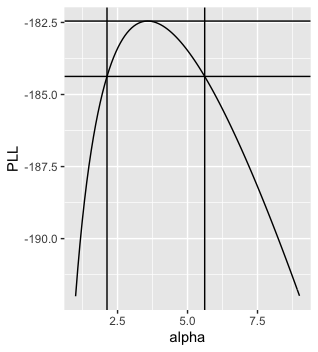
\includegraphics[width=1.5in]{a1/pll-alpha.png}}
\caption{Graph of the profile likelihood of $\alpha$ parameter in Gamma model}
\end{center}
\end{figure}
Let $\alpha_0$ be the true value of our alpha parameter. Using the profile deviance to create the confidence interval, we get \[\alpha_0\in [2.122419,5.612549]\]
Since 2 is not in this interval, we reject the null hypothesis.
\end{solution}


\end{document}

